Accediendo a la primera carpeta \textbf{1_YOLOV3} nos encontraremos con todos los scripts encargados de ejecutar el algoritmo. A su vez lo tenemos dividido en dos secciones: \textbf{OnlyYolo} y \textbf{YoloAndCNN}. \\
En la primera,\textbf{OnlyYolo}, tenemos cinco ficheros \textbf{Python}:

\begin{enumerate}
\item \textbf{imagen_yolov3.py}: script encargado de detección de señales en una imagen individual.
\item \textbf{video_yolov3.py}: script encargado de detección de señales en un video.
\item \textbf{camara_yolov3.py}: script encargado de detección de señales a través de la cámara frontal o webcam del ordenador.
\item \textbf{automatic_imagen_yolov3.py}: script encargado de detección de señales en una imagen individual, pero el nombre de la imagen a procesar se introducirá mediante línea de comandos y no dentro del fichero.
\item \textbf{automatizacion_imagenes.py}: script encargado de leer todas las imágenes de un directorio y mandárselas a través de línea de comandos al fichero \textit{automatic_imagen_yolov3.py} para poder procesar varias imágenes ininterrumpidamente.
\end{enumerate}

En la segunda sección denominada \textbf{YoloAndCNN} tendremos todos los ficheros más complejos que se han desarrollado para detectar cada señal de manera específica. Estos aplican al algoritmo de la primera sección una CNN (Red Neuronal Convolucional) para, por ejemplo, precisar que la señal de otros se trata de una señal de stop. Nos encontramos con los siguientes ficheros:
\begin{itemize}
\item \textbf{imagen_yolov3.py}: fichero que contiene todas las clases de señales con las que ha sido entrenado el modelo y que va a ser capaz de detectar.
\item \textbf{yolov3_ts_test.cfg}: fichero que contiene la configuración de \textbf{YOLO}.
\item \textbf{yolov3_ts.weights}: fichero que contiene los pesos obtenidos como resultado del entrenamiento del modelo.
\end{itemize}

En el script \textbf{imagen_yolov3.py} deberemos modificar la variable \textit{imageName} con el nombre de la imagen en formato JPG, que ha de encontrarse dentro del directorio destinado a las imágenes \textit{images}. Con el siguiente comando podemos visualizar un ejemplo, figura \ref{detecc1} 

\begin{lstlisting}
python3 imagen_yolov3.py
\end{lstlisting}

\begin{figure}[H]
	\centering
	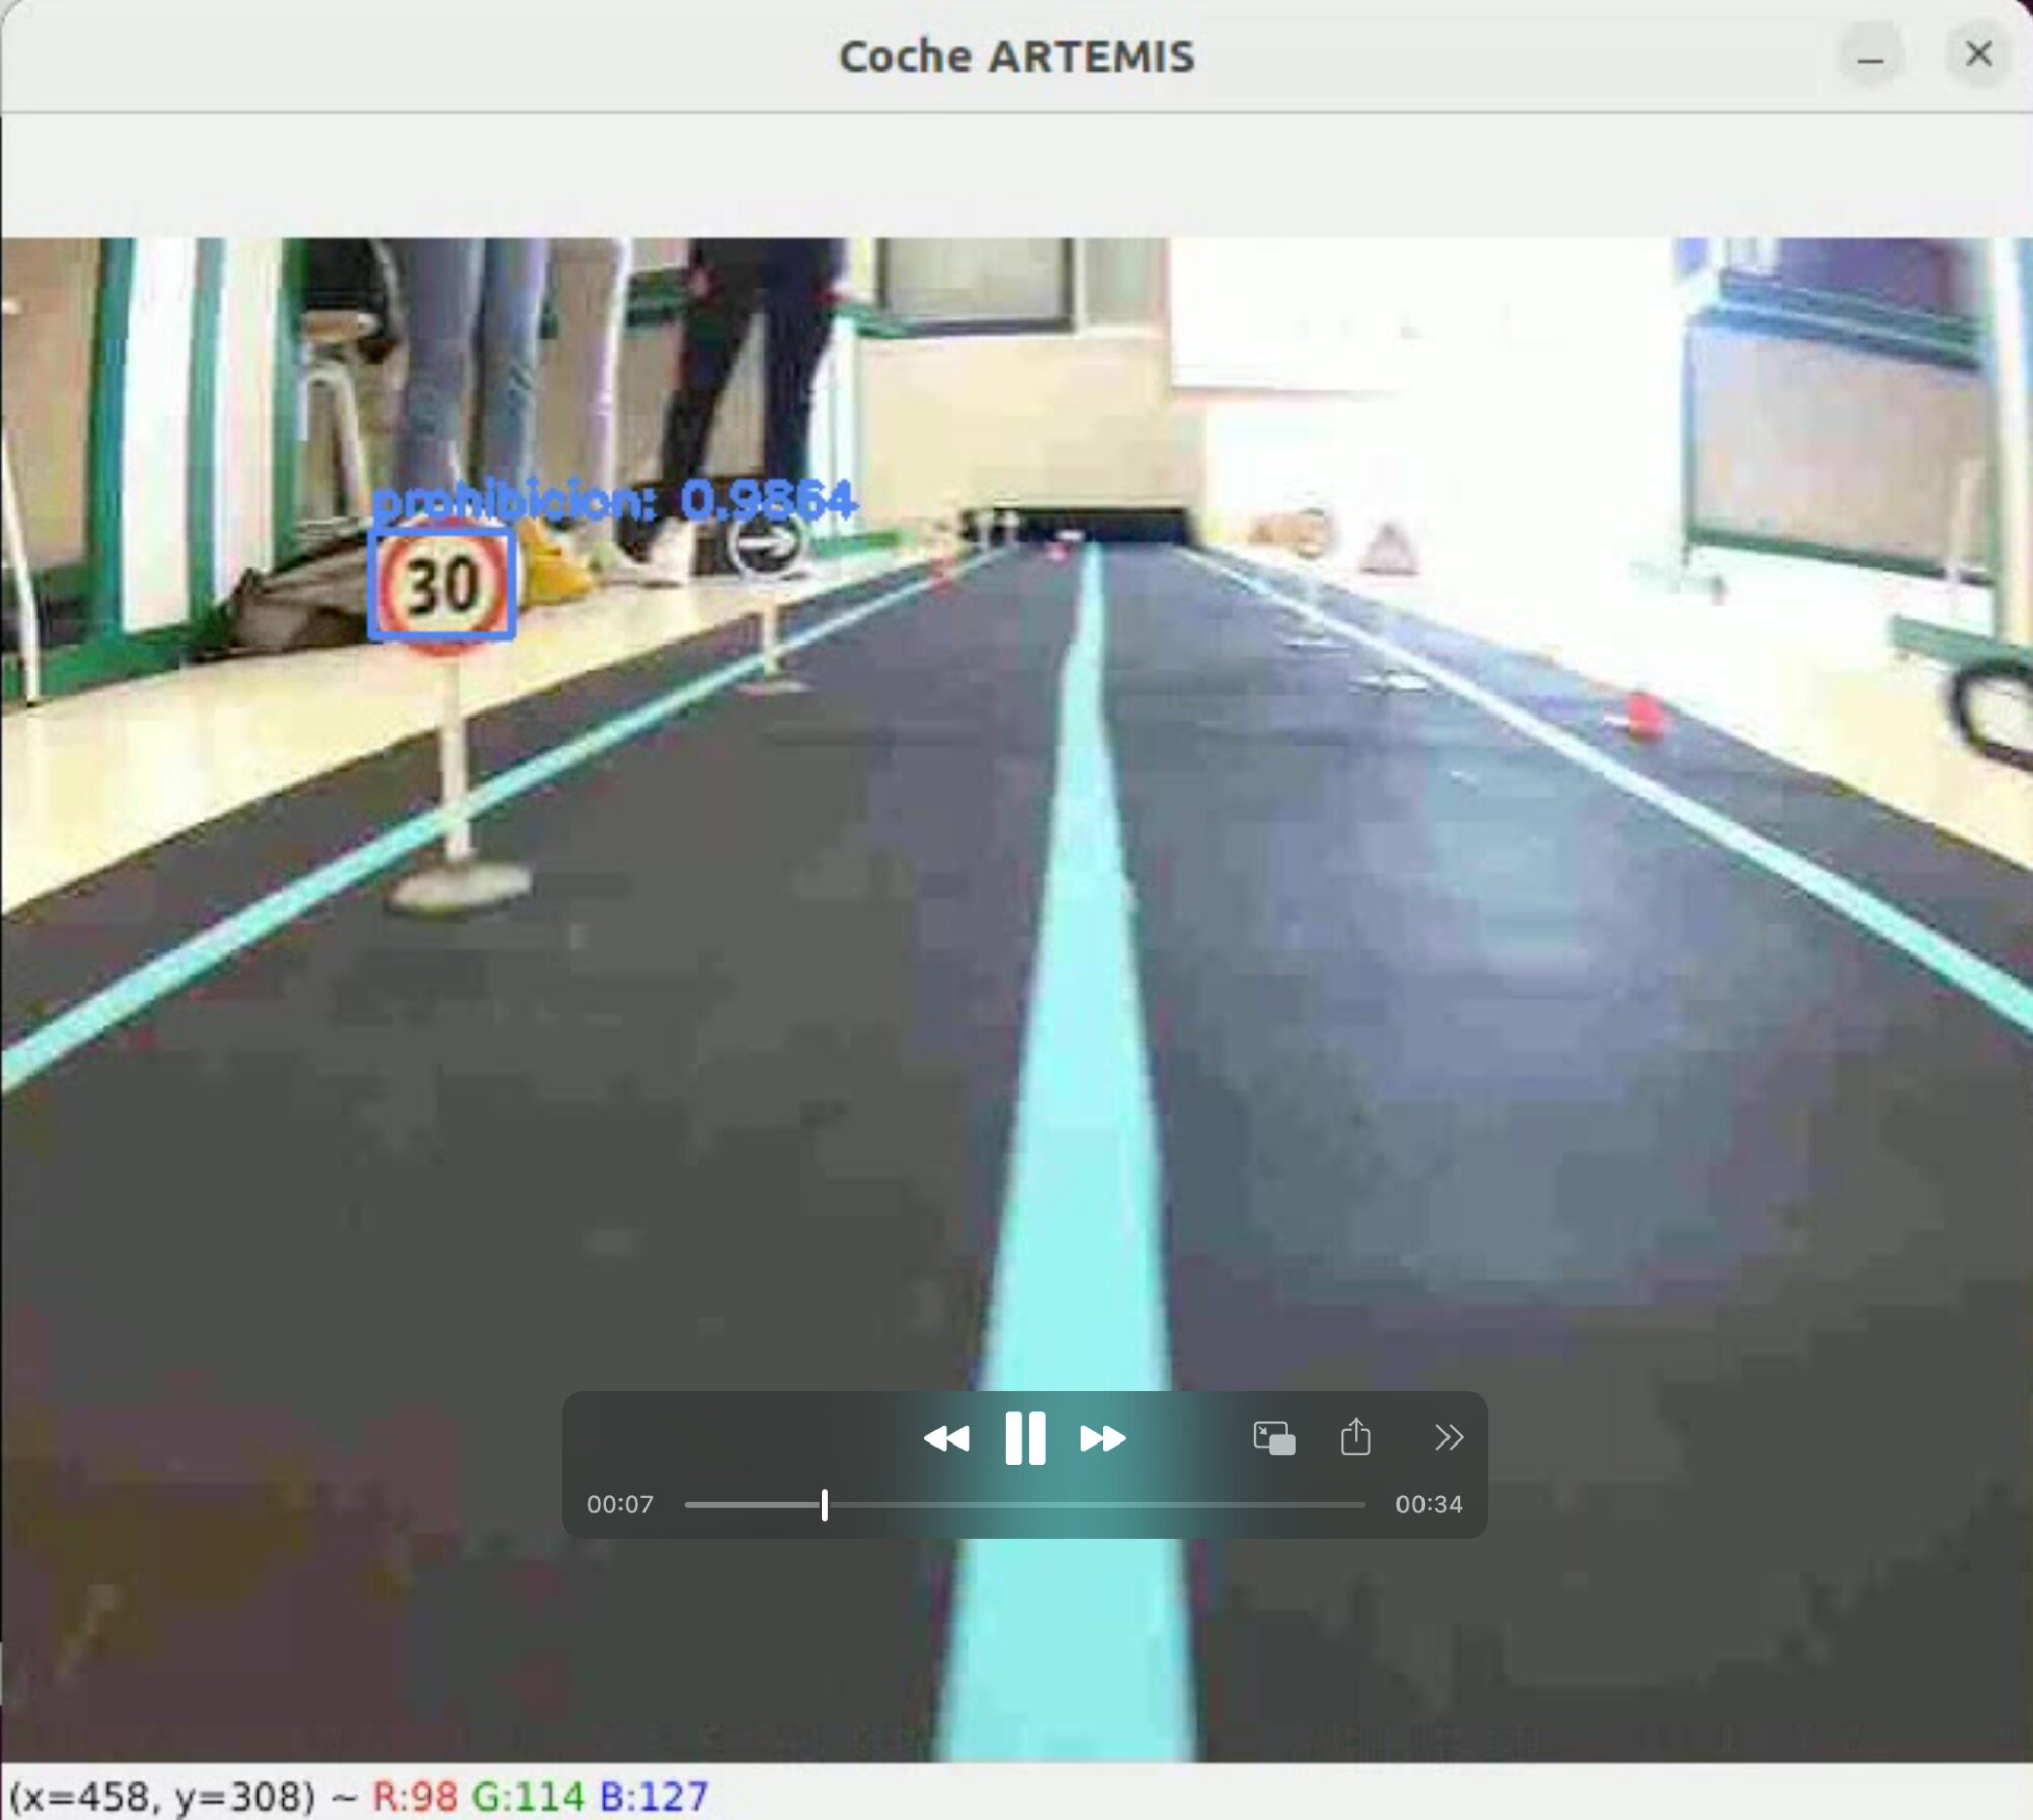
\includegraphics[width=\textwidth]{Imagenes/AnexoI_Manual/AA/deteccion1.pdf}
	\caption{Detección de una señal}
	\label{detecc1}
\end{figure}

En caso de querer realizar el procesamiento de un video, lo haremos con el script \textbf{yolo-3-video.py}. De igual manera debemos modificar la variable \textit{videoName} con el nombre del video, el cual ha de encontrarse dentro de la carpeta \textit{videos} en formato MP4. Lo pondremos en marcha mediante, obteniendo como resultado la figura \ref{detecc2}
\begin{lstlisting}
	python3 video_yolov3.py
\end{lstlisting}
	
\begin{figure}[H]
	\centering
	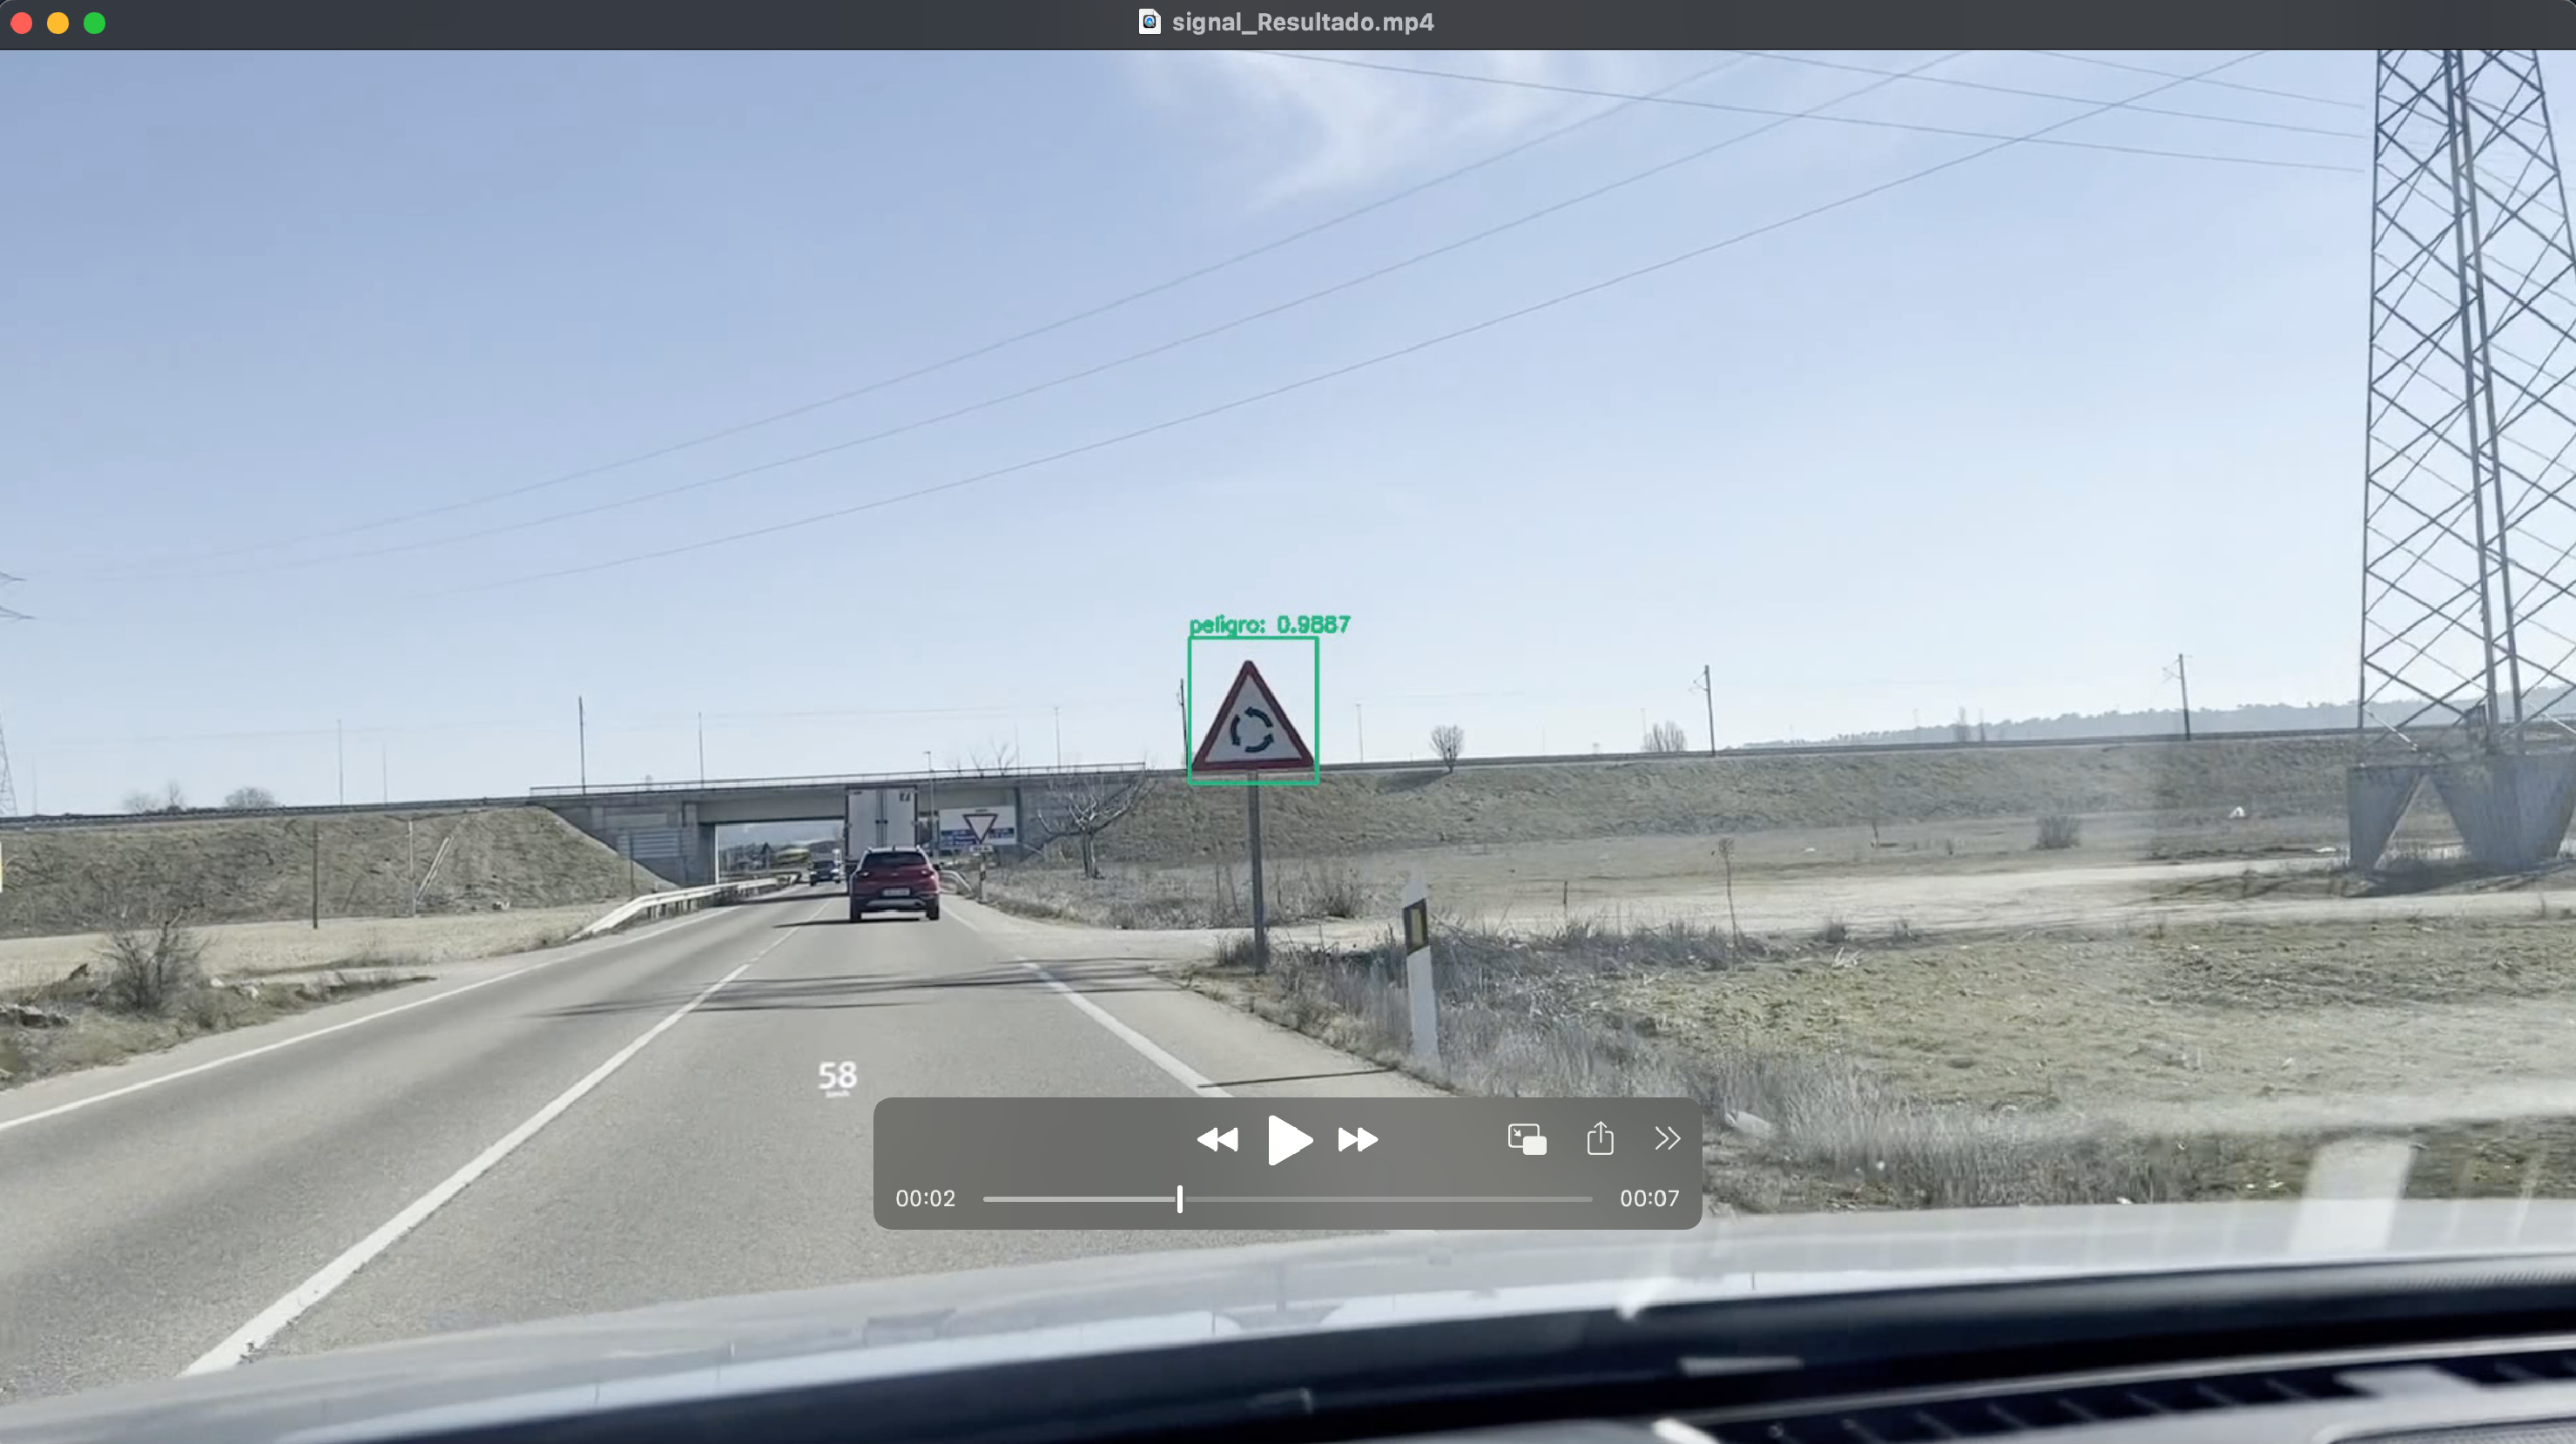
\includegraphics[width=\textwidth]{Imagenes/AnexoI_Manual/AA/deteccion2.pdf}
	\caption{Detección de una señal real capturada por nosotros}
	\label{detecc2}
\end{figure}

Asimismo, podremos procesar video en tiempo real procedente de la cámara o webcam de nuestro propio ordenador, figura \ref{detecc3}. A través del script \textbf{camara_yolov3.py} podremos ponerlo en marcha:

\begin{lstlisting}
python3 camara_yolov3.py
\end{lstlisting}

\begin{figure}[H]
	\centering
	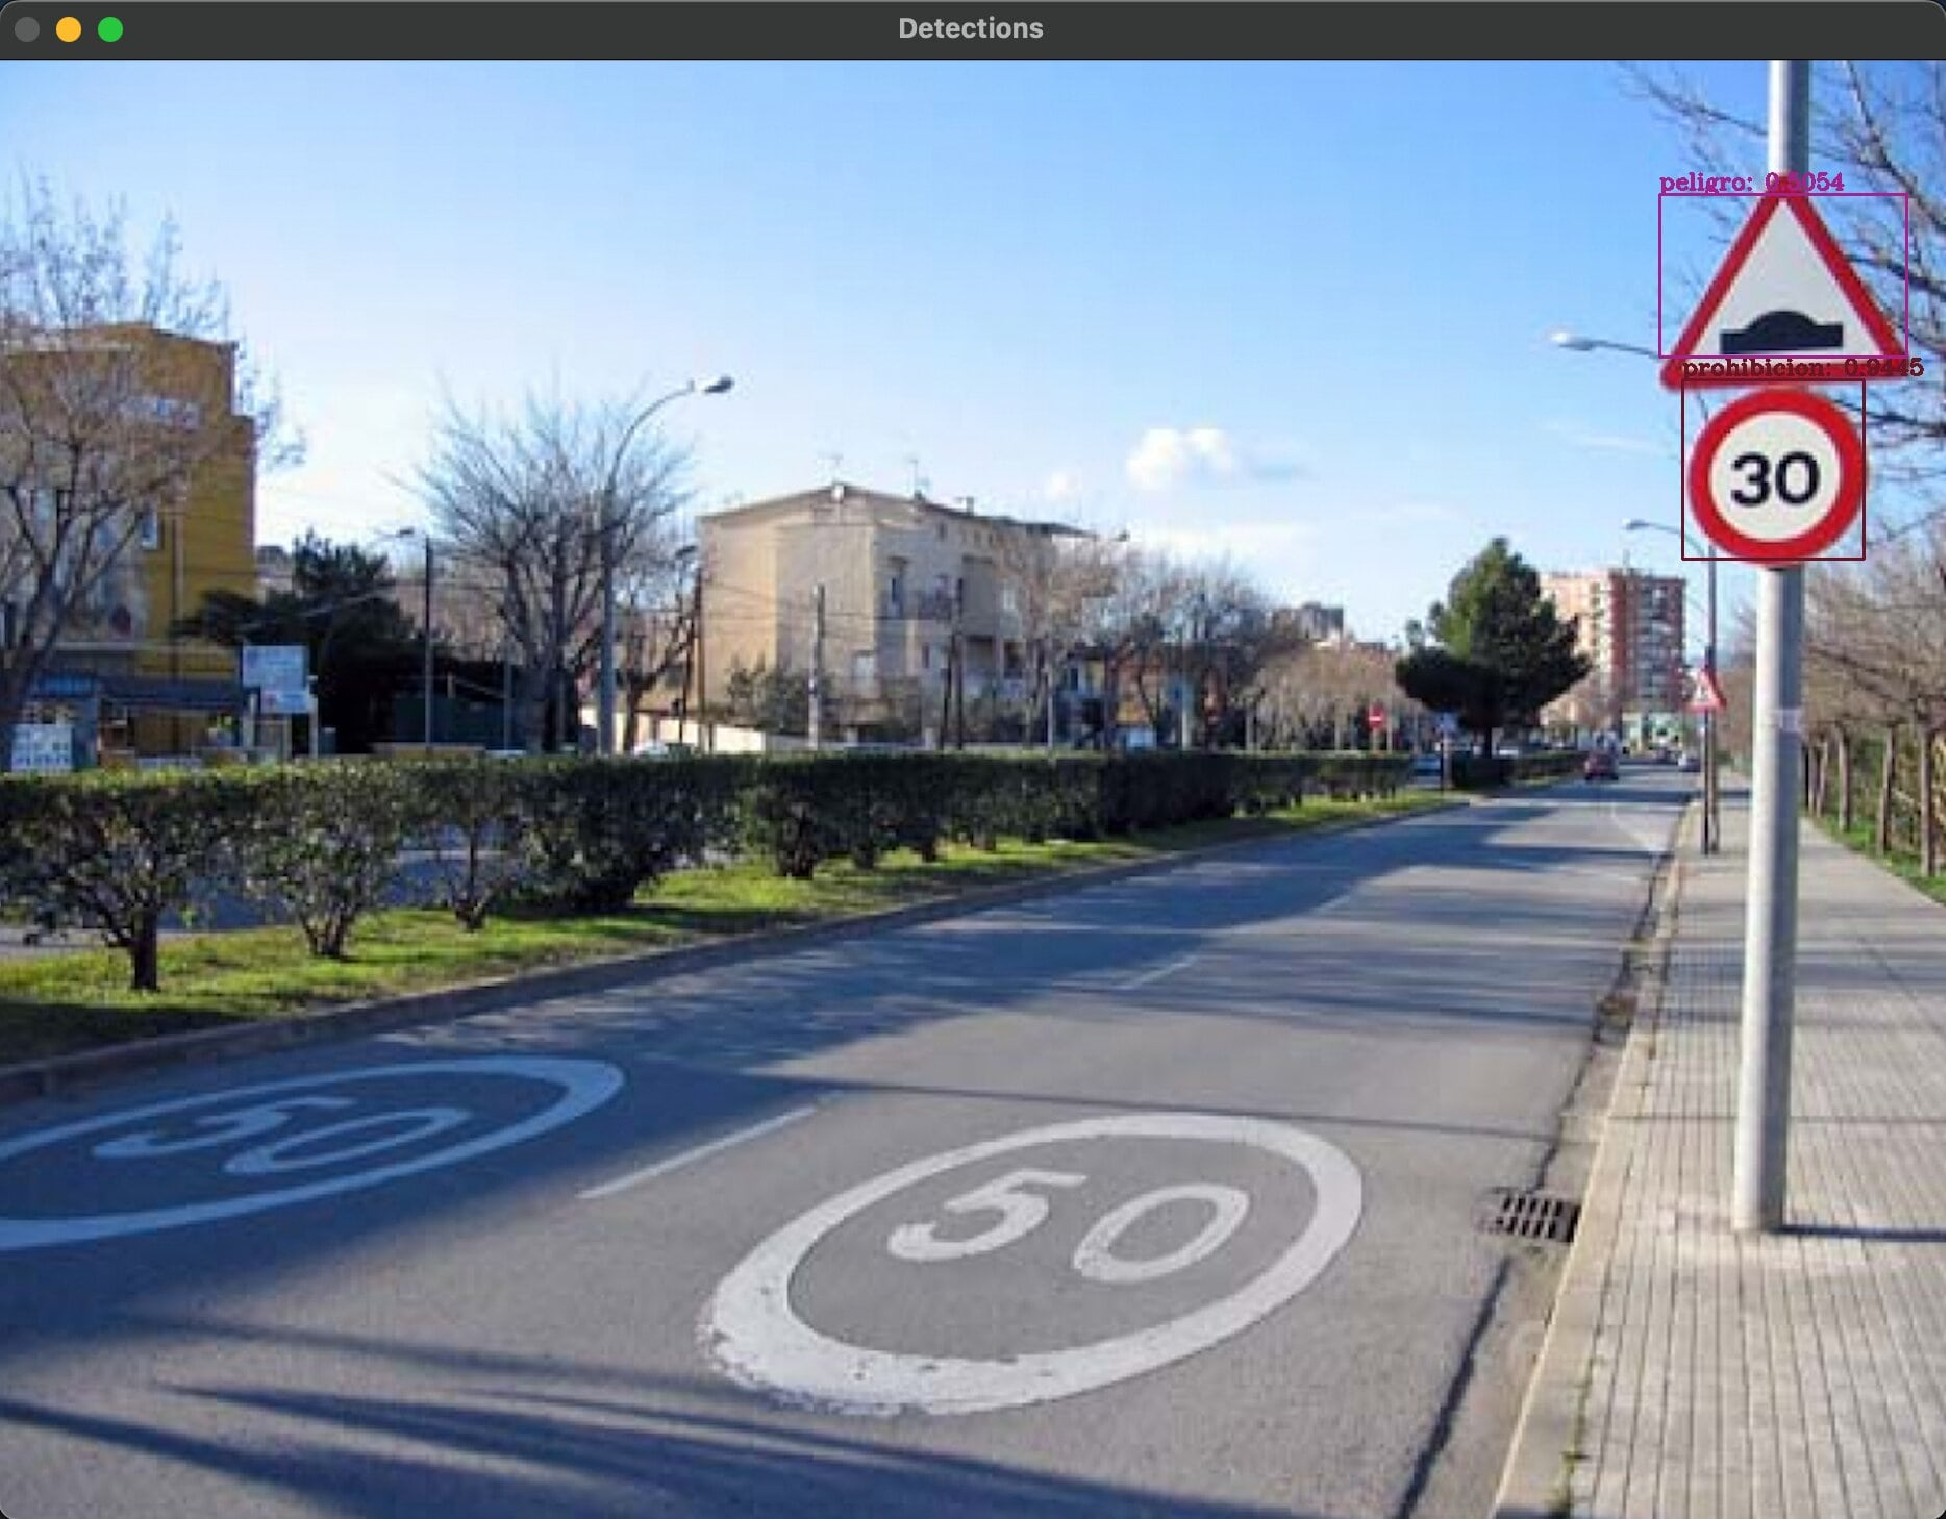
\includegraphics[width=\textwidth]{Imagenes/AnexoI_Manual/AA/deteccion3.pdf}
	\caption{Detección de una señal captada por la cámara}
	\label{detecc3}
\end{figure}

Puede ser de utilidad poder procesar muchas imágenes de manera conjunta, por ejemplo, si quisiéramos medir el rendimiento de la red. Para ello, disponemos de dos scripts que funcionan de manera conjunta, estos son \textbf{automatic_imagen_yolov3.py} y \textbf{automatizacion_imagenes.py}. 

El script que deberemos ejecutar es \textbf{automatizacion_imagenes.py}, el cual leerá cuáles son las imágenes que se encuentran en el directorio especificado en la variable \textit{directorioAutomatic} y ejecutará individualmente \textbf{automatic_imagen_yolov3.py} con el nombre de cada imagen como parámetro de entrada.

Dado que nosotros hemos utilizado dichos scripts para hacernos más sencilla la tarea de medición de rendimiento de la red, tendremos la posibilidad de crear un fichero \textbf{nombre_imagen.txt} por cada imagen, que contendrá las coordenadas del cuadro delimitador del objeto detectado y la precisión obtenida. Mediante la variable que se encuentra al comiendo del fichero \textbf{automatic_imagen_yolov3.py} llamada \textit{medirRendimientoRed} podremos controlar dos modos de operación:

\begin{itemize}
\item Si \textit{medirRendimientoRed} es \textbf{False}: su funcionamiento será análogo al script \textbf{imagen_yolov3.py}, pero podremos visualizar varias imágenes de seguido, simplemente deberemos pulsar cualquier tecla para visualizar la siguiente. 

\item Si \textit{medirRendimientoRed} es \textbf{True}: podremos crear el fichero \textbf{nombre_imagen.txt} con su información correspondiente dentro del directorio \textit{detections} para cada una de las imágenes, pero no iremos viendo en tiempo real el procesado.
\end{itemize}

Mediante la siguiente instrucción podremos ejecutarlo:

\begin{lstlisting}
python3 automatizacion_imagenes.py
\end{lstlisting}

Si además tuviéramos la opción de \textit{medirRendimientoRed} establecida a \textbf{True}, obtendremos un resultado similar al de la figura \ref{detecc4}.

\begin{figure}[H]
	\centering
	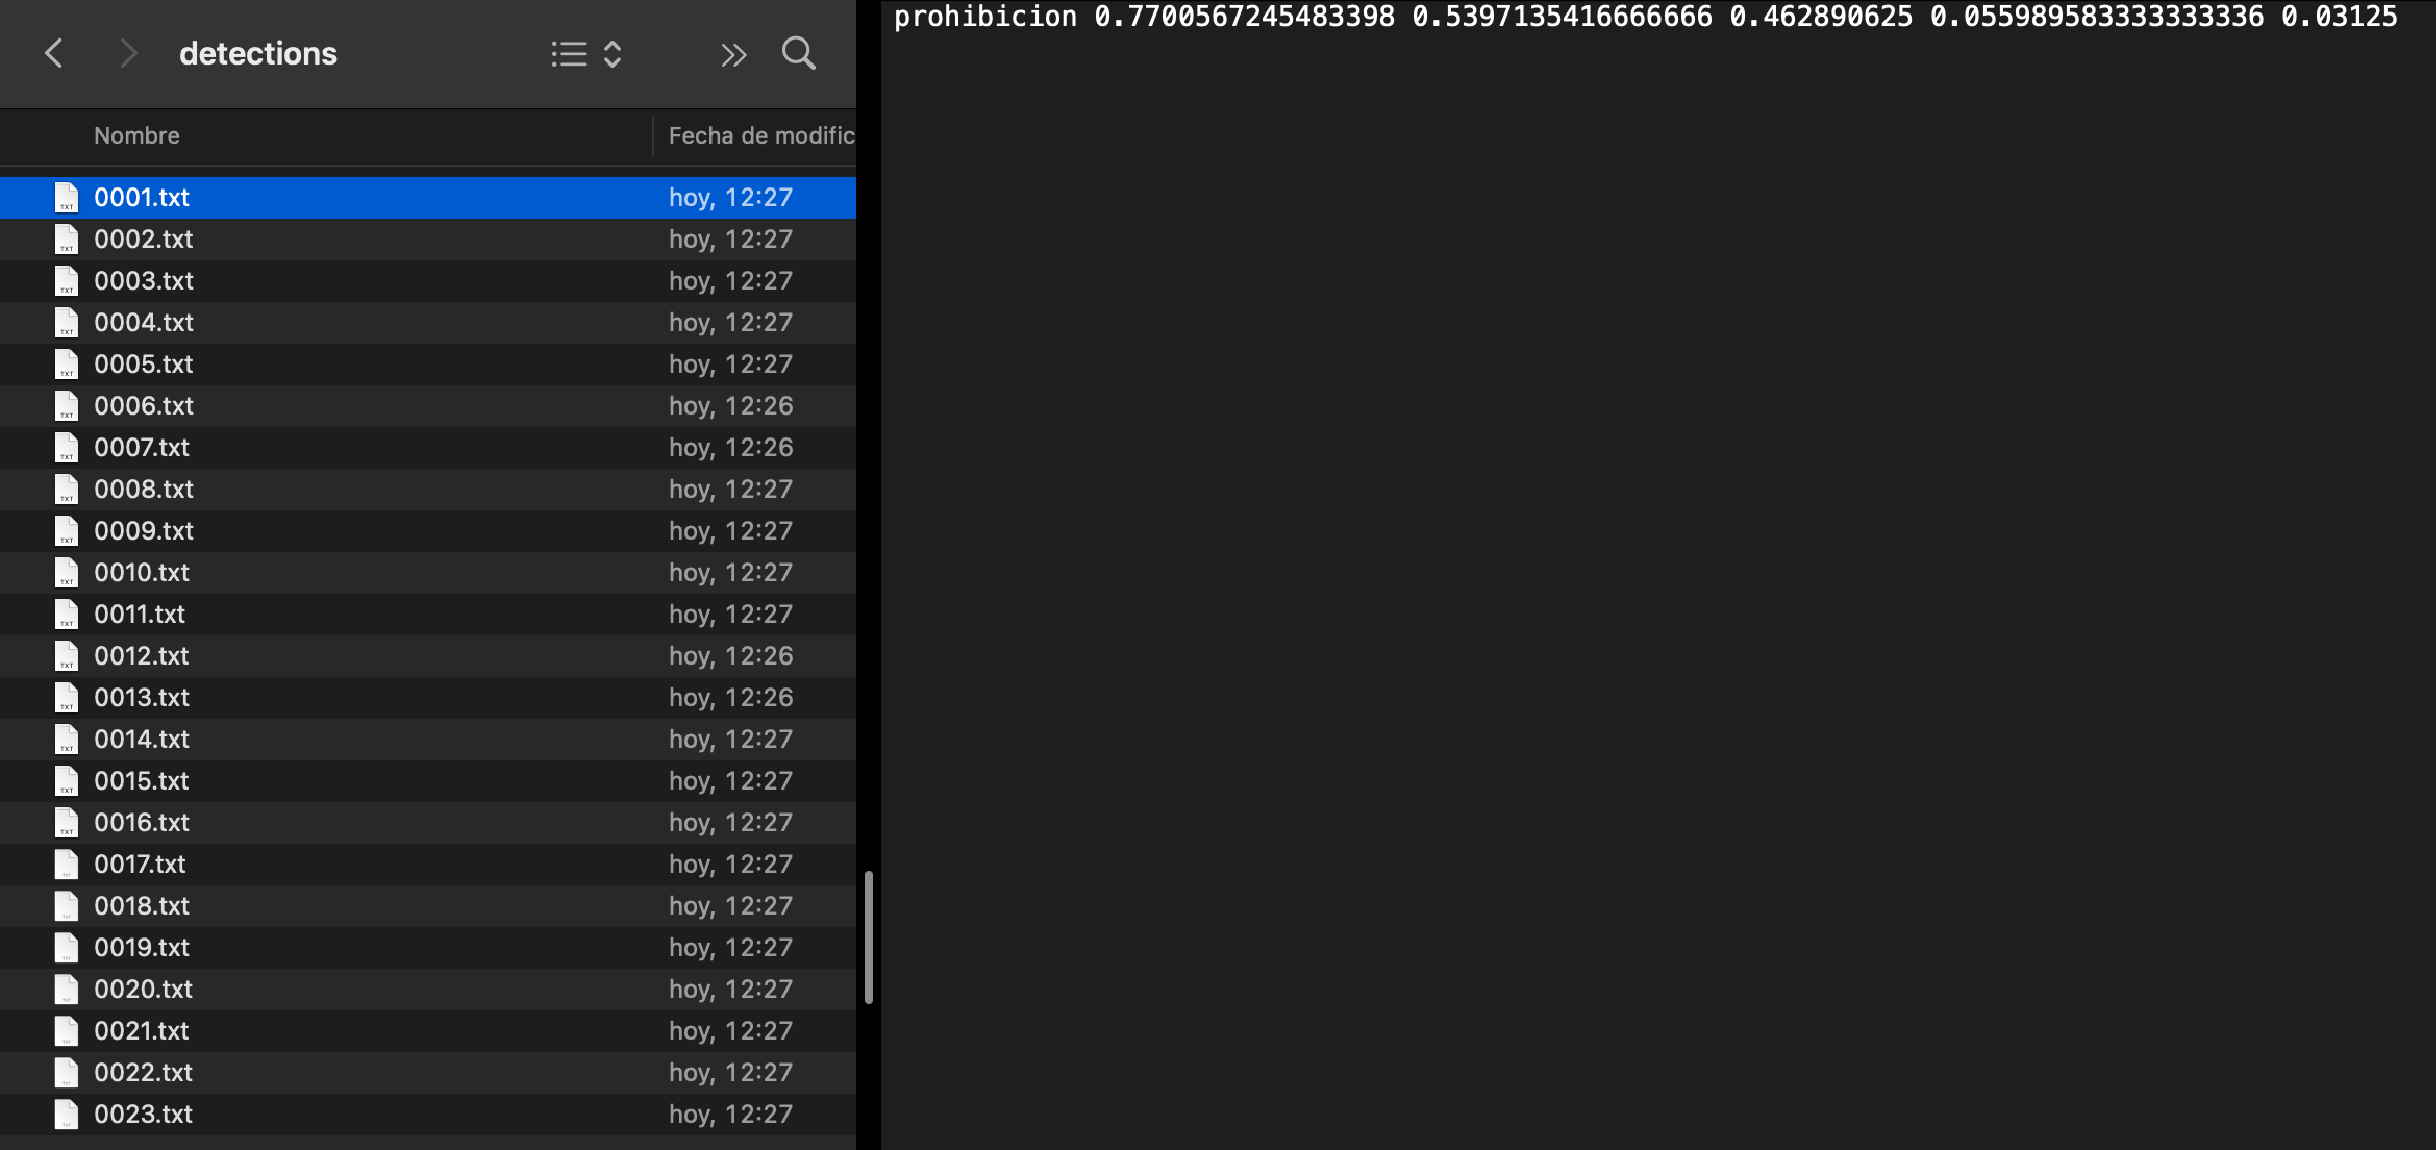
\includegraphics[width=\textwidth]{Imagenes/AnexoI_Manual/AA/deteccion4.pdf}
	\caption{Ejemplo de rendimiento con $medirRendimientoRed \ =\ True$}
	\label{detecc4}
\end{figure}


